\documentclass[12pt]{beamer}
\usetheme{Warsaw}
\usepackage[utf8]{inputenc}
\usepackage{amsfonts}
\usepackage{amsmath}
\usepackage{siunitx}
\usepackage{amssymb}
\usepackage{mathtools}
\usepackage[brazil]{babel}
\usepackage{geometry}
\usepackage{graphicx}
\usepackage{bussproofs}
\usepackage{gensymb}
\usepackage{hyperref}
\graphicspath{ {.} }
\linespread{1.5}
\newcommand{\real}{\mathbb{R}}
\newcommand{\product}[3]{\displaystyle\prod_{#1}^#2 #3}
\newcommand{\gsum}[3]{\displaystyle\sum_{#1}^#2 #3}
\newcommand{\mytitle}[1]{\textbf{\underline{#1}}}
\newcommand{\ring}[1]{\langle#1\rangle}
\newcommand{\code}[1]{\mbox{\texttt{#1}}}

\setbeamertemplate{headline}{}
\title{Apresentação EP2 Redes (2021)}
\author{Lourenço Sborz (11208005) \& Mohamad Rkein (10740130)}

\date{\today}

\begin{document}

\begin{frame}
  \titlepage{}
\end{frame}
\begin{frame}
  \tableofcontents
\end{frame}

\section{Protocolo}

\subsection{Início da Conexão}
\begin{frame}
  Depois que o cliente conecta com o servidor, a primeira coisa que o servidor faz é usar o socket dessa conexão para enviar duas novas portas para o cliente. Uma dessas portas será usada para abrir a conexão criptografada e a outra será usada para abrir a conexão que chamamos de \textit{background server listener}. A conexão criptografada e a conexão normal são usadas para enviar para o servidor os comandos manuais que o usuário escreveu na prompt. O \textit{background server listener} é usado por uma thread separada e fica o tempo todo recebendo e respondendo pings, além de ser responsável por verificar se o usuário foi ``desafiado''.
\end{frame}

\subsection{Comandos}
\begin{frame}
  Os comandos digitados pelos usuários são parseados da seguinte maneira: primeiro, quebramos o comando nos espaços, para separar os argumentos do nome e depois checamos por qual socket o comando deve ser enviado. Por exemplo, se o usuário digtou \texttt{login a b}, sabemos que isso deve ser enviado pelo socket criptografado, então enviamos o comando e seus argumentos pelo socket com SSL. Se o comando não existe, enviamos ele pelo socket criptografado. Fizemos isso por dois motivos:
\end{frame}
\begin{frame}
  \begin{enumerate}
    \item Achamos melhor tratar os erros no servidor, pois um usuário malicioso poderia simplesmente modificar o seu cliente para deixar as falhas passarem caso elas fosse tratadas dentro do código do cliente.
    \item Já que vamos enviar os comandos errados para o servidor pelo motivo anterior, é melhor enviarmos eles pelo criptografado, pois pode ser que o cliente tenha escrito \textit{logn username passw}.
  \end{enumerate}
\end{frame}
\begin{frame}
  Todos os comandos enviados pelo cliente têm algum tipo de resposta do servidor, nem que seja um simples ``ok'', indicando que tudo ocorreu corretamente.
\end{frame}
\begin{frame}
  Alguns comandos só estão habilitados para o usuário usar em condições específicas, por exemplo: o usuário só pode usar o comando begin se ele está logado.
\end{frame}

\subsection{Jogo}
\begin{frame}
  O jogo é feita de maneira \textit{peer to peer} como exigido no enunciado. Suponhamos dois usuários: a e b. O que acontece quando a desafia b usando o comando \texttt{begin b} é: o begin é enviado para a thread do servidor responsável por a. Essa thread se comunica com a thread o servidor responsável por b usando o algoritmo dos produtores e consumidores e então a thread responsável por b envia esse comando para o cliente do b. b pode então digitar \texttt{refuse} ou \texttt{accept} (nesse caso é enviado junto uma porta e o IP de b) para responder. A resposta de b faz o caminho inverso que o begin fez, e chega até o a, que então age da maneira adequada. No caso de \texttt{refuse}, o a simplesmente recebe a mensagem de que seu pedido foi recusado e no caso de \texttt{accept} a conexão \textit{p2p} é estabelecida e então o jogo é começado.
\end{frame}

\subsection{Tratamento de Erros}
\begin{frame}
  Como pedido no enunciado, implementamos um sistema de heartbeat. O servidor envia um pacote de ``Ping'' para o cliente a cada 3 segundos. O cliente irá assumir que sua conexão foi interrompida caso ele fique 3 minutos sem receber o ping e irá fechar os sockets e imprimir uma mensagem de erro. O servidor faz a mesma coisa, caso não receba resposta do ping em 3 minutos, ele irá assumir que o cliente caiu e irá fechar a conexão com o cliente.
\end{frame}
\begin{frame}
  Quando o servidor é finalizado com SIGKILL, os clientes ficam 3 minutos tentando reconectar. Caso o servidor seja reiniciado na mesma porta dentro desse intervalo, os clientes são reconectados automaticamente e os que estava logados, são logados automaticamente também. Caso os 3 minutos passem sem o servidor ser reiniciado, os clientes avisam o usuário e terminam. Consideramos que o servidor servidor foi finalizado com uma falha se ele morreu enquanto ainda tinha algum usuário logado.
\end{frame}

\section{Extras}
\subsection{IA}
\begin{frame}
  Como bônus, implementamos um cliente (\texttt{cliente\_ia.py}) que é uma inteligência artificial que (teoricamente) nunca perde. Para jogar contra ela basta conectá-la no servidor e desafiar o usuário chamado ``velha''.
\end{frame}

\section{Experimentos e Gráficos}
\subsection{Sem clientes}
\begin{frame}
  Uso de cpu e memória para o servidor sem clientes:
  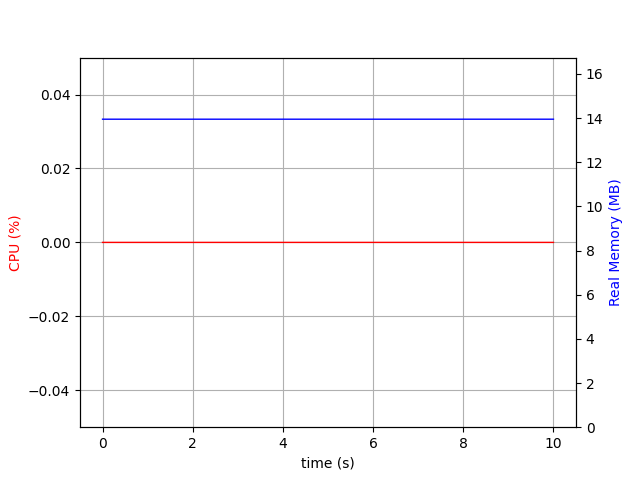
\includegraphics[scale=0.6]{./servidorsolo.png}
\end{frame}
\subsection{Com 2 clientes sem jogar}
\begin{frame}
  Uso de cpu e memória para o servidor com 2 clientes sem jogar:
  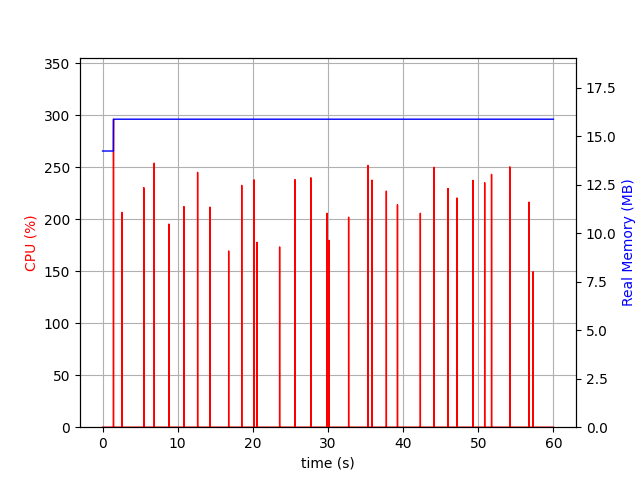
\includegraphics[scale=0.6]{./servidorsemjogar.png}
\end{frame}
\subsection{Com 2 clientes jogando}
\begin{frame}
  Uso de cpu e memória para o servidor com 2 clientes jogando:
  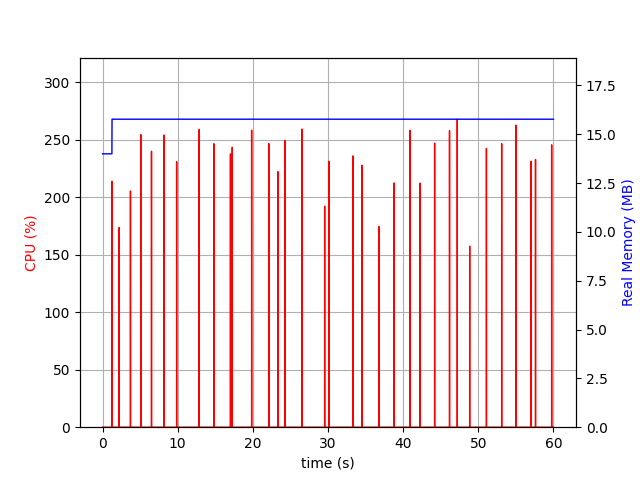
\includegraphics[scale=0.6]{./servidorjogando.png}
\end{frame}
\subsection{Comparação do uso de rede nos testes}
\begin{frame}
  Uso de rede em bytes para os testes:
  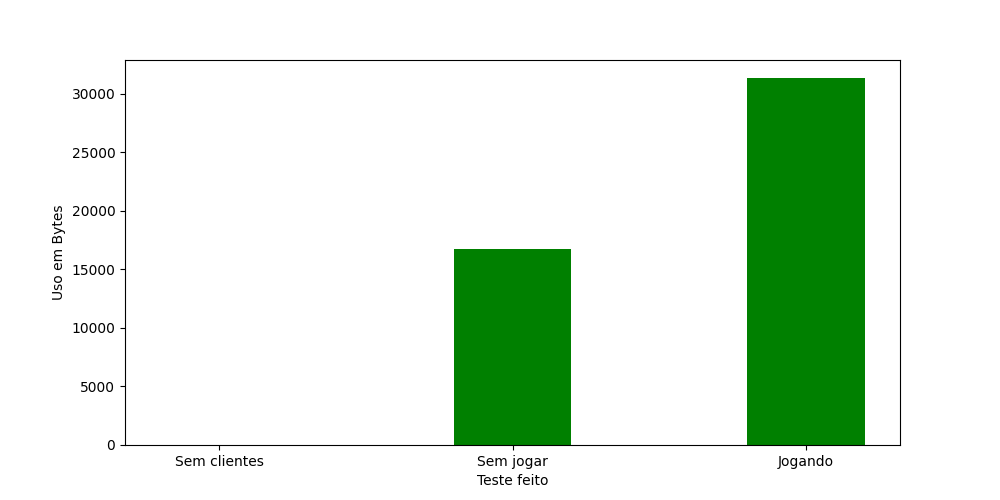
\includegraphics[scale=0.427]{./grafico.png}
\end{frame}

\subsection{Conclusão}
\begin{frame}
  Com os gráficos podemos perceber que o uso de cpu do servidor foi quase o mesmo no caso onde os clientes jogavam e no caso onde eles não jogavam. Isso se deve ao fato de que toda a implementação da lógica do jogo é client-side. Além disso fica claro que sem clientes, o servidor fica basicamente parado, ou seja, o uso de cpu e rede ficam constantes e baixos. O uso de memória está alto em todos os casos, pois como o programa foi feito em python, sempre que importamos uma biblioteca todo o seu código é executado e é exatamente isso que constitui o uso relevante de memória do nosso programa, fazendo com que a variância entre os casos de teste seja pequena.
\end{frame}
\begin{frame}
  O uso de rede quase dobra quando os clientes jogam entre si, pois além do heartbeat com o servidor, precisamos também ficar mandando pings entre os clientes. Em todos os casos, a maior parte do uso de rede se deve aos pings.
\end{frame}
\end{document}